\documentclass[a4paper, 12pt]{article}

% srpski jezik, utf8
\usepackage[serbian]{babel}
\usepackage[utf8]{inputenc}

% podrska za graficke elemente
\usepackage{graphicx}

% podrska za margine i sl.
\usepackage{geometry}

% podrska za boje
\usepackage{xcolor}

% podrska za stavljanje hyperlink-ova u sadrzaj
\usepackage{hyperref} 
\hypersetup{
	colorlinks	= true,
	citecolor	= cyan!90!black,
	linkcolor	= cyan!90!black,
	urlcolor	= cyan!90!black
}

% podesavanja fonta
\newcommand{\thefont}{Myriad Pro}

\usepackage{mathspec}
\setmathsfont(Digits)[Numbers={Lining,Proportional}]{\thefont}
\setmathsfont(Latin)[Numbers={Lining,Proportional}]{\thefont}
\setmathsfont(Greek)[Numbers={Lining,Proportional}]{\thefont}
\setmathrm{\thefont}

\usepackage{polyglossia}
\setmainlanguage[Script=Latin]{serbian}
\setotherlanguage{english}
\newfontfamily{\serbianfont}[Script=Latin, Language=Serbian]{\thefont}
\newfontfamily{\serbianfonttt}{\thefont}
\newfontfamily{\englishfont}[Language=English]{\thefont}
\newfontfamily{\englishfonttt}{\thefont}

% promena standardnih imena:
%     Bibliografija -> Literatura
\renewcommand{\refname}{Literatura}

% za [H] u figure
\usepackage{float} 

% za vertikalno spajanje celija u tabeli
\usepackage{multirow}

% za redefinisanje izgleda numerisanih listi
\renewcommand{\labelenumii}{\theenumii.}
\renewcommand{\theenumii}{\theenumi.\arabic{enumii}}
\renewcommand{\theenumiii}{\theenumii.\arabic{enumiii}}

% za rotiranje stranica
\usepackage{pdflscape}

% za podesavanje hedera i futera
\usepackage{fancyhdr}

% okruzenje za landscape
\newenvironment{mylandscape}
{
	\newpage
	\pagestyle{plain}
	
	\paperwidth=\pdfpageheight
	\paperheight=\pdfpagewidth
	\pdfpageheight=\paperheight
	\pdfpagewidth=\paperwidth
	
	\headwidth=\textheight
	
	\begingroup 
	
	\vsize=\textwidth
	\hsize=\textheight
}
{
	\endgroup
	\newpage
	
	\paperwidth=\pdfpageheight
	\paperheight=\pdfpagewidth
	\pdfpageheight=\paperheight
	\pdfpagewidth=\paperwidth
	
	\headwidth=\textwidth
	\newpage
}

% meta-informacije o tekstu
\author{Ajzenhamer Nikola 1083/2016\\Bukurov Anja 1082/2016\\Vojislav Stankovi\'c 1080/2016}
\title{INFORMACIONI SISTEM NACIONALNE SLU\v ZBE ZA ZAPO\v SLJAVANJE}
\date{\today}

\begin{document}

\begin{titlepage}
	\centering
	\noindent{\Large Matemati\v cki fakultet\\Univerzitet u Beogradu}
	
	\vspace{0.3\textheight}
	
	{\Huge INFORMACIONI SISTEM\\NACIONALNE SLU\v ZBE ZA ZAPO\v SLJAVANJE}
	\\~
	\\
	{\Large — timski projektni rad —}
	
	\vfill
	
	{
		\Large 
		\begin{tabular}{|l|l|l|}
			\hline
			\multirow{3}{*}{Studenti} & Ajzenhamer Nikola     & 1083/2016\\ \cline{2-3}
			                          & Bukurov Anja          & 1082/2016\\ \cline{2-3}
			                          & Stankovi\' c Vojislav & 1080/2016\\
			\hline
			Predmet                   & \multicolumn{2}{l|}{Informacioni sistemi}\\
			\hline
			\v Skolska godina         & \multicolumn{2}{l|}{2016/2017}\\
			\hline
			Nastavnik                 & \multicolumn{2}{l|}{dr Sa\v sa Malkov}\\
			\hline
			Datum                     & \multicolumn{2}{l|}{\today}\\
			\hline
		\end{tabular}
	}
\end{titlepage}
\newpage
\tableofcontents
\newpage

\section{Uvod}

Ovaj rad se bavi modeliranjem dela sistema Nacionalne slu\v zbe za zapo\v sljavanje republike Srbije. U okviru ovog rada, obra\' cena je pa\v znja i na mogu\' ca unapre\dj enja sistema.\\

Rad je izra\dj en kao timski studentski projekat na Matemati\v ckom fakultetu, na studijskom programu Informatika, prve godine Master studija. Projekat je odra\dj en pod nadzorom profesora dr Sa\v se Malkova, u okviru predmeta Informacioni sistemi.\\

U nastavku \' cemo detaljnije opisati rad Nacionalne slu\v zbe.

\subsection{Nacionalna slu\v zba za zapo\v sljavanje}

Nacionalna slu\v zba za zapo\v sljavanje (u daljem tekstu Nacionalna slu\v zba) obavlja poslove zapo\v sljavanja, osiguranja za slu\v caj nezaposlenosti, ostvarivanje prava iz osiguranja za slu\v caj nezaposlenosti i druga prava u skladu sa zakonom, odnosno poslove vo\dj enja evidencija u oblasti zapo\v sljavanja, kao i stru\v cno-organi\-zacione, upravne, ekonomsko-finansijske i druge op\v ste poslove u oblasti zapo\v sljavanja i osiguranja za slu\v caj nezaposlenosti, u skladu sa zakonom, svojim statutom i drugim aktima Nacionalne slu\v zbe.

\begin{mylandscape}
	\subsubsection{Dijagram konteksta}
	
	\begin{figure}[H]
		\centering
		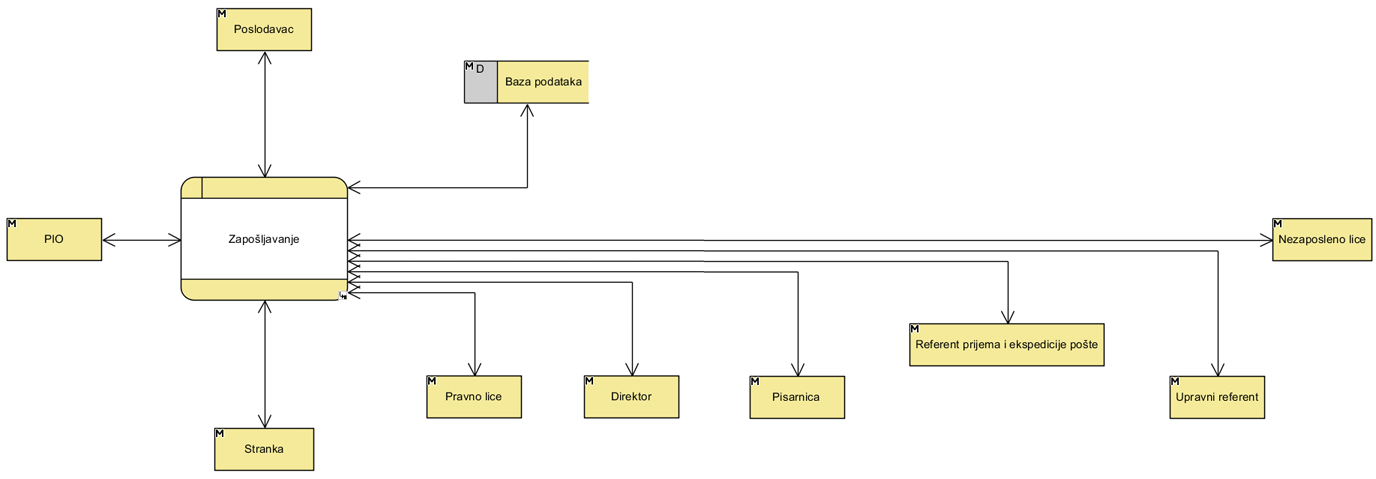
\includegraphics[width=0.8\paperwidth]{dijagrami/dijagrami-toka-podataka/zaposljavanje-dijagram-konteksta.png}
		\caption{Dijagram konteksta — prikaz sistema kao proces ''Zapo\v sljavanje''.}
		\label{dtp: dijagram konteksta}
	\end{figure}

	\newpage
	
	\begin{figure}[H]
		\centering
		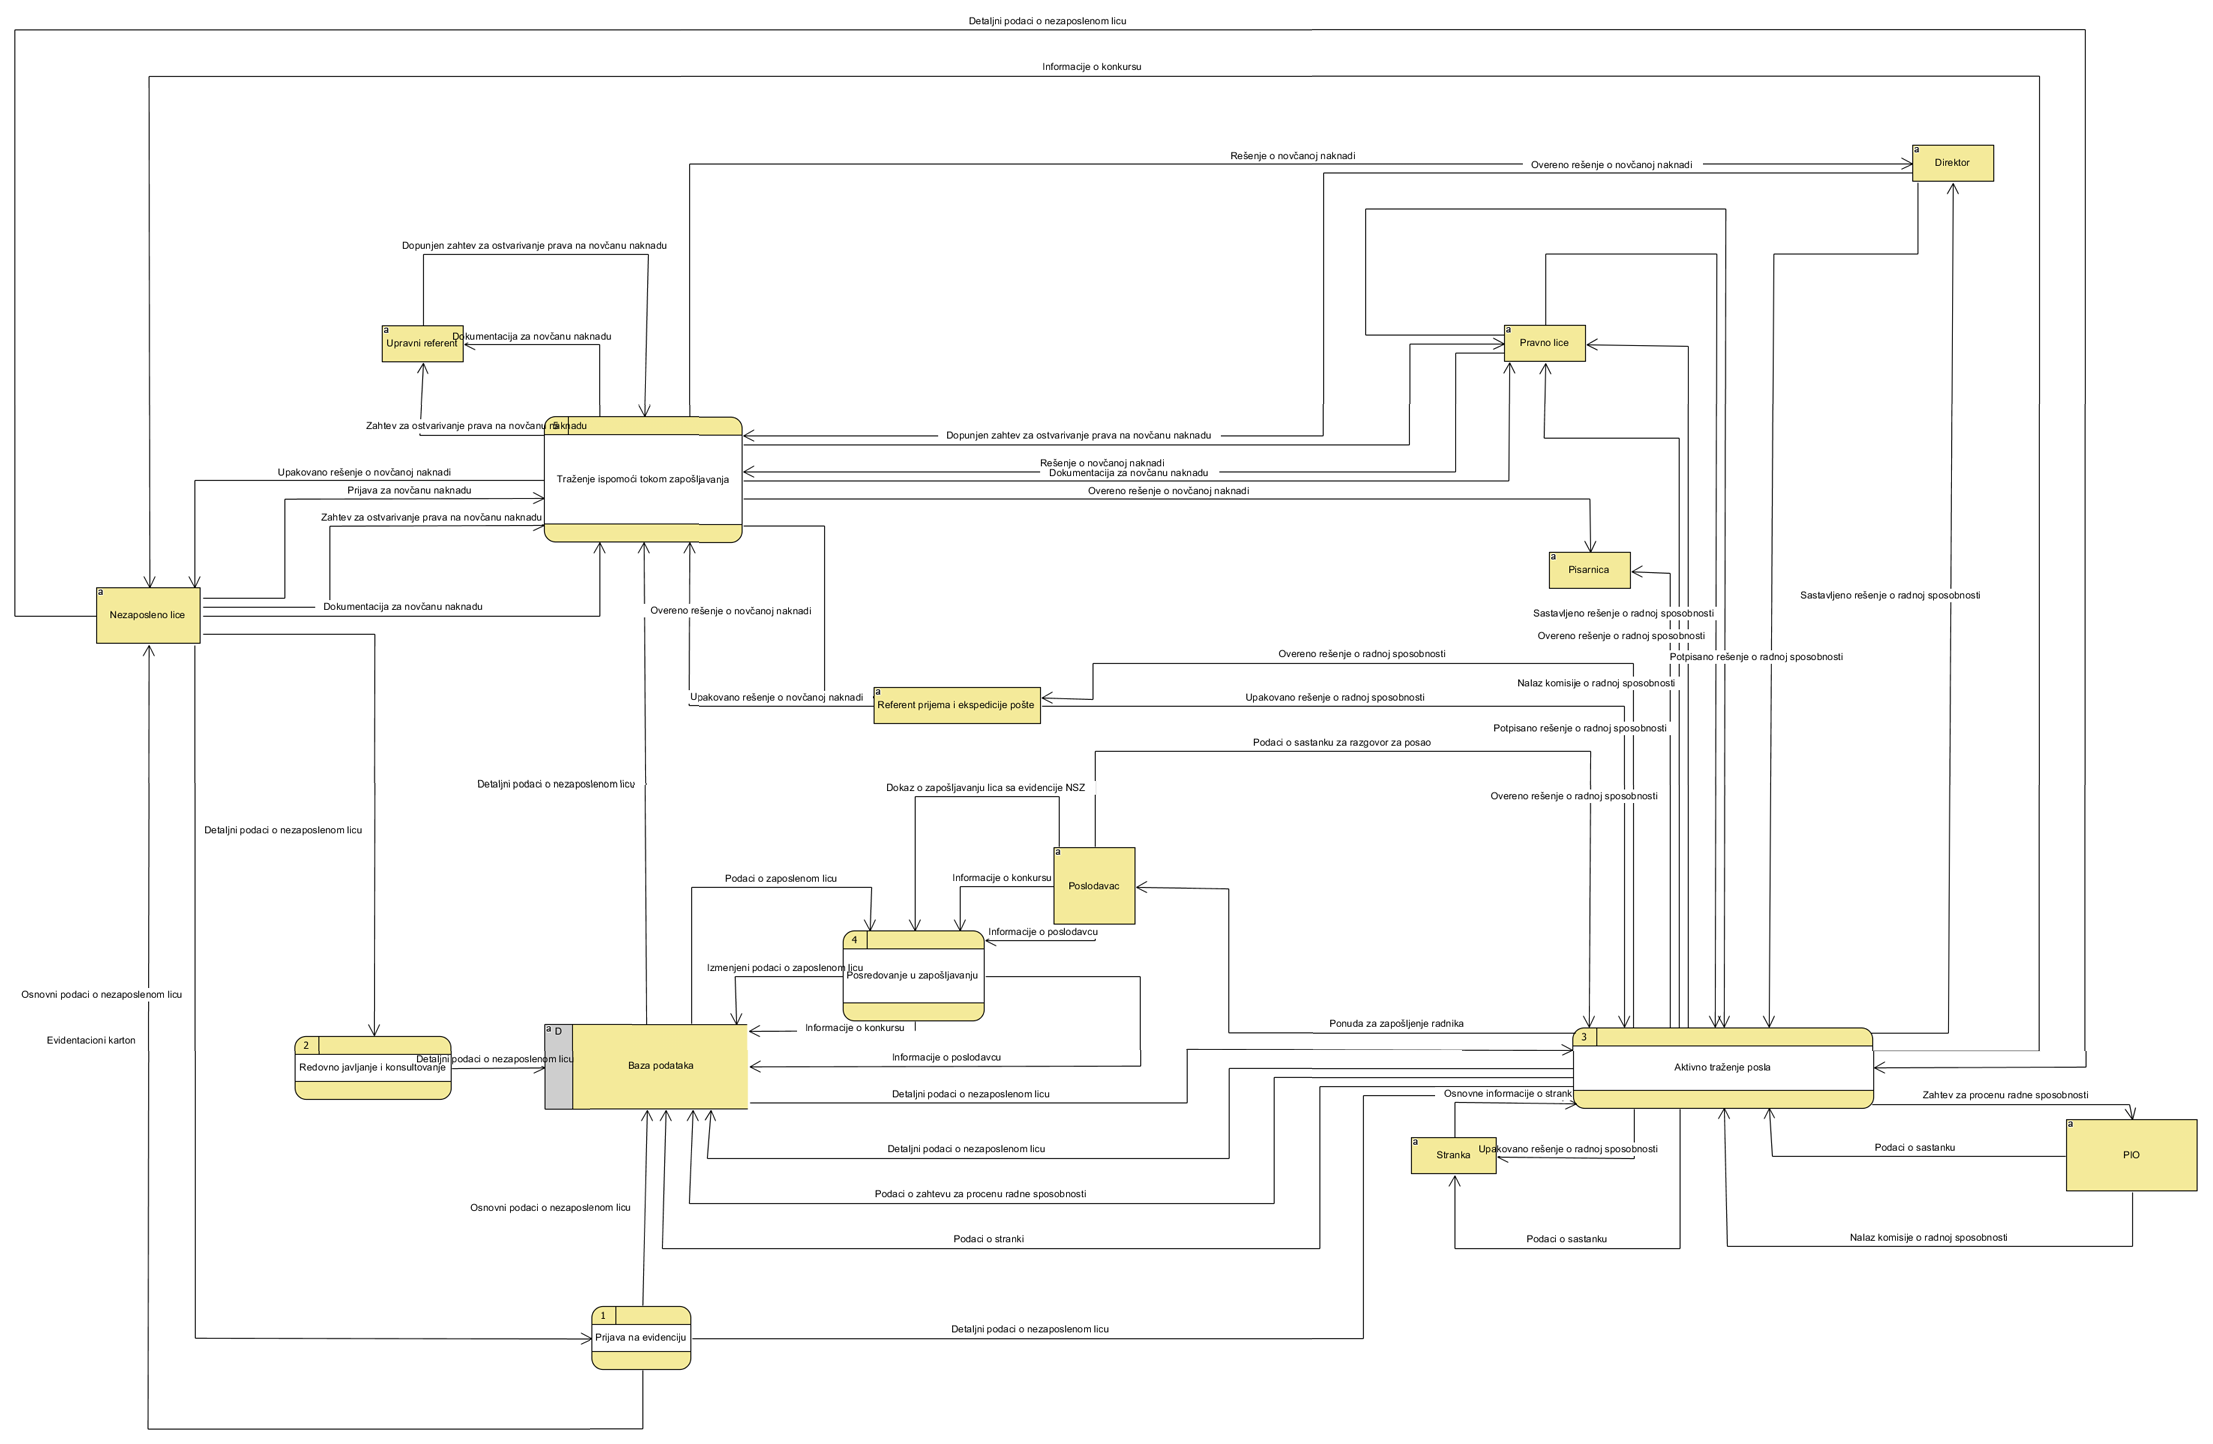
\includegraphics[width=0.7\paperwidth]{dijagrami/dijagrami-toka-podataka/zaposljavanje-dtp-nivoa-0.png}
		\caption{Dekompozicija procesa ''Zapo\v sljavanje'' (Slika \ref{dtp: dijagram konteksta}).}
	\end{figure}

\end{mylandscape}

\subsection{Metodologija rada}

Prilikom izrade rada, informacije o Nacionalnoj slu\v zbi su prikupljene iz dva glavna izvora. Prvi izvor predstavljaju zvani\v cna dokumenta Nacionalne slu\v zbe, i to ''Program rada Nacionalne slu\v zbe za zapo\v sljavanje (za 2016. godinu)'' i ''Statut Nacionalne slu\v zbe za zapo\v sljavanje'', \v cijim razmatranjem smo dolazili do formalnih informacija o sistemu. Drugi izvor informacija je razgovor sa zaposlenim licima, \v sto nam je prevashodno omogu\' cilo da steknemo uvid u mogu\' ca unapre\dj enja sistema.\\

Deo sistema koji je analiziran je modeliran kori\v s\' cenjem razli\v citih dijagramskih tehnika. U daljem tekstu \'cemo navesti kori\v s\'cene tehnike i dati ukratke opise.\\

Zahtevi sistema su modelirani dijagramima slu\v cajeva upotrebe (engl. \textit{Use Case Diagram}). Slu\v caj upotrebe je niz koraka pona\v sanja (scenario), automatskih i ru\v cnih, koji slu\v ze za kompletiranje jednog poslovnog zadatka. Dijagram slu\v cajeva upotrebe prikazuje interakciju izme\dj u sistema i eksternih sistema i korisnika. Drugim re\v cima, on grafi\v cki predstavlja ko \' ce koristiti sistem i na koje na\v cine korisnik mo\v ze da interaguje sa sistemom (\cite{SADM}). Dijagrami slu\v cajeva upotrebe su dopunjeni BPMN dijagramima i dijagramima sekvence.\\

\textit{Business Process Model and Notation} (skra\' ceno, BPMN) standard je za modeliranje poslovnih procesa koji obezbe\dj uje grafi\v cku notaciju za preciziranje poslovnih procesa. Cilj BPMN je da podr\v zi modeliranje poslovnih procesa za tehni\v cke i netehni\v cke (poslovne) korisnike nude\' ci notaciju koja je intuitivna poslovnim licima, a opet dovoljno jaka da mo\v ze da predstavi kompleksnu procesnu semantiku (\cite{BPMN}). Dakle, BPMN dijagrame (posebno, BPMN dijagrame saradnji) koristi\' cemo za opisivanje interakcije izme\dj u entiteta tokom slu\v cajeva upotrebe.\\

Dijagrami sekvence (engl. \textit{Sequence Diagram}) ilustruju objekte koji u\v cestvuju u slu\v caju upotrebe i poruke koje se razmenjuju izme\dj u njih u toku vremena, u jednom slu\v caju upotrebe (\cite{SAAD}). Ove dijagrame \' cemo koristiti pri slu\v cajevima upotrebe za koje smatramo da je potrebno dodatno opisati tok scenarija u vremenu.\\

Dijagram stanja (engl. \textit{state diagram} ili \textit{state machine diagram}) predstavlja dinami\v cki model koji prikazuje razli\v cita stanja kroz koje jedna klasa prolazi tokom svog \v zivota (\cite{SAAD}).\\

Dijagrami toka podataka (engl. \textit{Data Flow Diagrams}) predstavljaju jednu od osnovnih tehnika strukturnih metodologija. DTP opisuju na koji na\v cin se kre\' cu podaci kroz sistem. Razlikujemo nivoe DTP, pa tako dijagram konteksta predstavlja DTP najvi\v seg nivoa i njime se \v citav sistem (podsistem) predstavlja kao jedan proces (\cite{smalkov-slajdovi}). Dijagram konteksta \' cemo koristiti upravo da bismo pokazali granice sistema i komunikaciju sa njegovim okru\v zenjem.\\

Dijagram klasa (engl. \textit{Class Diagram}) predstavlja stati\v cki model koji podr\v zava stati\v cki pogled sistema u razvoju. On prikazuje klase i odnose izme\dj u klasa koje ostaju nepromenljive u sistemu tokom vremena (\cite{SAAD}).\\

Kao softversko re\v senje za izradu pomenutih dijagrama, kori\v s\' cen je Visual Paradigm 14.\\

Veliki broj opisanih slu\v cajeva upotrebe sadr\v zi rukovanje sa sistemom, pa zbog toga, u okviru ovog rada, obra\' cena je i pa\v znja na projektovanje korisni\v ckog interfejsa. Kao pristup izrade prototipa (engl. \textit{prototyping}) korisni\v ckog interfejsa odabran je HTML prototip.\\

HTML prototip se izgra\dj uje kori\v s\'cenjem Veb stranica napisanih u HTML (engl. \textit{HyperText Mark-up Language}) jeziku. Postupak podrazumeva kreiranje serije Veb stranica koje pokazuju fundamentalne delove sistema. Korisnici mogu da interaguju sa stranicama klikom na dugmad i uno\v senjem podataka u formulare (naravno, po\v sto nema sistema u pozadini, podaci se ne procesuiraju). Stranice su povezane tako da, kada korisnik klikne na dugmad, prikazuje se zahtevani deo sistema (\cite{SAAD}).

\newpage
\section{Slu\v cajevi upotrebe}

Slu\v caj upotrebe je celina posla koja daje nekakav smisleni rezultat, a dovoljno je mala da mo\v ze da se jednozna\v cno opi\v se i implementira \cite{smalkov-slajdovi}.\\

Opis slu\v caja upotrebe bi trebalo da bude dovoljno duga\v cak, tj. da obuhvati sve ono \v sto je potrebno da bi neko mogao na osnovu tog opisa da napravi ta\v cnu implementaciju. Svaki slu\v caj upotrebe mora da ima svoj opis \cite{smalkov-slajdovi}.\\

Ve\' cina UML dijagrama se zasniva prvenstveno na grafi\v ckom obliku. Dijagram slu\v cajeva upotrebe predstavlja odnose slu\v cajeva upotrebe i aktera. Pojedinosti slu\v cajeva upotrebe se opisuju tekstualno. Dobar opis slu\v caja upotrebe sadr\v zi dovoljno informacija da se mo\v ze sagledati kada, kako, ko i sa kojim podacima u\v cestvuje u slu\v caju upotrebe \cite{smalkov-slajdovi}.

\subsection{Prijava na evidenciju}

Nezaposleno lice dolazi li\v cno u Nacionalnu slu\v zbu za zapo\v sljavanje radi prijave na evidenciju. U zavisnosti od toga da li je lice ve\' c bilo na evidenciji ili ne razlikujemo dva slu\v caja:

\begin{itemize}
	\item ukoliko lice nije bilo nikada ranije prijavljeno na evideniciji, izvr\v sava se slu\v caj upotrebe Prva prijava (\ref{su: prva prijava})
	\item ukoliko je lice bilo prijavljeno na evidenciju ali je izgubilo status aktivnog tra\v zenja posla zbog neredovnog javljanja izvr\v sava se slu\v caj upotrebe Ponovna prijava (\ref{su: ponovna prijava}).
\end{itemize}

\begin{figure}[H]
	\centering
	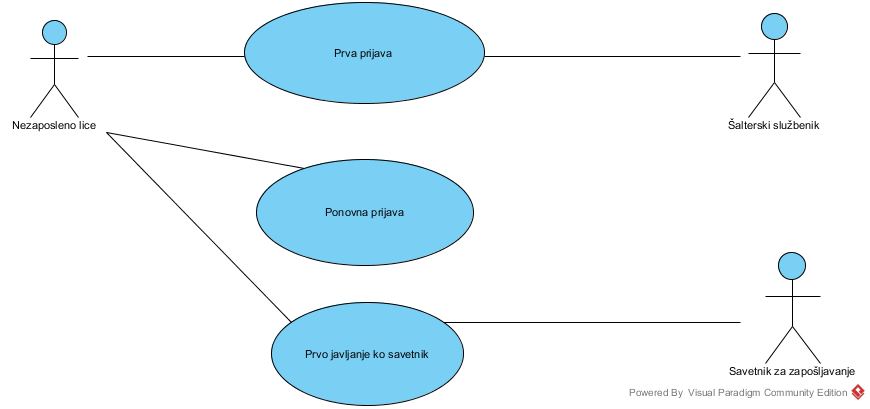
\includegraphics[width=0.8\textwidth]{dijagrami/dijagrami-slucajeva-upotrebe/prijava-na-evidenciju.png}
	\caption{Dijagram slu\v cajeva upotrebe - Prijava na evidenciju}
	\label{dsu: prijava na evidenciju}
\end{figure}

\subsubsection{Slu\v caj upotrebe: Prva prijava}
\label{su: prva prijava}

\noindent U\v cesnici: Nezaposleno lice (u daljem tekstu NL), \v salterski slu\v zbenik (u daljem tekstu \v SS)
\\
\\ Preduslovi: NL ima li\v cnu kartu i dokaz o stru\v cnoj spremi. Automat za izdavanje broja je u funkciji. \v SS je ulogovan na sistem. 
\\
\\ Postuslovi: NL je ili uspe\v sno prijavljen na evidenciju i izdat je evidencioni karton tra\v zioca zaposlenja, ili mu je ukazano na njegov status.
\\
\\ Glavni tok:
\begin{enumerate}
	\item NL prilazi automatu i bira opciju ''Prijava na evidenciju''.
	\item Automat bele\v zi da je opcija ''Prijava na evidenciju'' odabrana, ra\v cuna naredni broj u redu \v cekanja za tu opciju, i \v stampa papir sa brojem.
	\item NL uzima broj i \v ceka svoj red.
	\item Kada do\dj e na red, NL prilazi \v salteru i zahteva od \v SS da ga prijavi na evidenciju.
	\item \v SS otvara formular za prijavu.
	\item \v SS tra\v zi od NL da mu preda li\v cnu kartu i dokaz o stru\v cnoj spremi.
	\item NL predaje potrebna dokumenta. 
	\item \v SS popunjava formular na osnovu predatih dokumenata.
	\item \v SS daje NL-u da popuni Obrazac za prijavu na evidenciju.
	\item NL popunjava Obrazac za prijavu na evidenciju, a zatim ga vra\' ca \v SS-u.
	\item \v SS popunjava Evidencioni karton za tra\v zioca zaposlenja.
	\item \v SS zakazuje prvo javljanje savetniku za zapo\v sljavanje, i postavlja status NL-a na ''aktivan''.
	\item \v SS vra\' ca dokumenta NL-u i daje mu evidentacioni karton.
	\item Prelazi se na slu\v caj upotrebe \ref{su: prvo javljanje savetniku}.
\end{enumerate}

\noindent Alternativni tokovi: 
\begin{description}
	\item[A1. Pad sistema] ~\\
	Ukoliko se u bilo kom koraku Glavnog toka dogodi pad sistema na kojem radi \v SS, \v SS ponovo pokre\'ce sistem i prijavljuje se na njega.
	\begin{enumerate}
		\item \v SS proverava da li je formular sa\v cuvan.
		\item Ukoliko jeste, prelazi se na korak 9 Glavnog toka.
		\item Ina\v ce, prelazi se na korak 8 Glavnog toka.
	\end{enumerate}

	\item[A2. Status NL-a je ''zamrznut''] ~\\
	Ukoliko u koraku 8 Glavnog toka sistem prika\v ze da postoje informacije o NL-u, kao i da je njegov status ''zamrznut'', \v SS obave\v stava NL-a o njegovom statusu, i slu\v caj upotrebe se zavr\v sava.
\end{description}

\subsubsection{Slu\v caj upotrebe: Ponovna prijava}
\label{su: ponovna prijava}

\noindent  U\v cesnici: Nezaposleno lice (u daljem tekstu NL), \v salterski slu\v zbenik (u daljem tekstu \v SS)
\\
\\ Preduslovi: NL ima li\v cnu kartu. Automat za izdavanje broja je u funkciji. \v SS je ulogovan na sistem. 
\\
\\ Postuslovi: NL-u je uspe\v sno promenjen status i izdat je novi evidencioni karton tra\v zioca zaposlenja.
\\
\\ Glavni tok:
\begin{enumerate}
	\item NL prilazi automatu i bira opciju ''Prijava na evidenciju''.
	\item Automat bele\v zi da je opcija ''Prijava na evidenciju'' odabrana, ra\v cuna naredni broj u redu \v cekanja za tu opciju, i \v stampa papir sa brojem.
	\item NL uzima broj i \v ceka svoj red.
	\item Kada do\dj e na red, NL prilazi \v salteru i zahteva od \v SS da mu promeni status.
	\item \v SS tra\v zi od NL da mu preda li\v cnu kartu.
	\item NL predaje li\v cnu kartu.
	\item \v SS pronalazi NL-a u sistemu. 
	\item \v SS bira opciju izmeni podatke.
	\item \v SS menja status "zamrznut" u "aktivan".
	\item \v SS popunjava Evidencioni karton za tra\v zioca zaposlenja.
	\item \v SS zakazuje prvo javljanje savetniku za zapo\v sljavanje, i postavlja status NL-a na ''aktivan''.
	\item \v SS vra\' ca dokumenta NL-u i daje mu evidentacioni karton.
	\item Prelazi se na slu\v caj upotrebe \ref{su: prvo javljanje savetniku}.
\end{enumerate}

\noindent Alternativni tok: /

\subsubsection{Slu\v caj upotrebe: Prvo javljanje savetniku}
\label{su: prvo javljanje savetniku}

\noindent U\v cesnici: Nezaposleno lice (u daljem tekstu NL), savetnik za zapo\v sljavanje (SZ)
\\
\\ Preduslovi: NL ima evidentacioni karton. SZ je ulogovan na sistem. 
\\
\\ Postuslovi: Ili je uspe\v sno zabele\v zeno javljanje NL-a ili je postavljen status NL-a na ''zamrznut''.
\\ 
\\ Glavni tok:
\begin{enumerate}
	\item NL dolazi kod SZ-a u kancelariju i predaje mu svoj evidentacioni karton.
	\item SZ pronalazi NL-a u sistemu.
	\item SZ i NL razgovaraju o NL-ovoj stru\v cnoj spremi, kakvi poslovi zanimaju NL-e, i koje ve\v stine Nl poseduje.
	\item SZ unosi nove informacije u sistem.
	\item SZ tra\v zi informacije o prethodnim zaposlenjima NL-a, i ako postoje i te informacije, SZ ih unosi u sistem.
	\item SZ zakazuje slede\' ce javljanje i vra\' ca NL-u evidentacioni karton.
\end{enumerate}

\noindent Alternativni tok:
\begin{description}
	\item[A1. Promena statusa NL-a na ''zamrznut''] ~\\
	Ukoliko u koraku 1 Glavnog toka NL ne do\dj e na prvo javljanje pre zakazanog termina, automatski se \v salje zahtev za izmenom podataka o NL-u u sistemu, i to: status NL-a se prebacuje na ''zamrznut''. Slu\v caj upotrebe se zavr\v sava.
\end{description}
\subsection{Kori\v s\' cenje onlajn sistema Nacionalne slu\v zbe}

Onlajn sistem Nacionalne slu\v zbe je veb aplikacija koja omogu\' cava obavljanje odre\dj enih poslovnih funkcija vezanih za eksterne korisnike putem interneta. Kori\v s\' cenjem onlajn sistema, eksterni korisnici mogu uz manje napora i br\v ze da dobiju usluge Nacionalne slu\v zbe.\\

Onlajn sistem prepoznaje dve vrste eksternih korisnika: \textit{nezaposleno lice}, i \textit{predstavnik kompanije sa kojom Nacionalna slu\v zba sara\dj uje} (radi jednostavnosti, ovaj subjekat \'cemo nazivati \textit{kompanija}). Na Slici \ref{dsu: koriscenje onlajn sistema nacionalne sluzbe} prikazani su navedeni korisnici i procesi u kojima u\v cestvuju, a koje \'cemo opisati u daljem tekstu.\\

Za oba korisnika je omogu\' ceno pravljenje naloga i prijavljivanje na sistem. Pravljenje naloga za nezaposlena lica i kompanije je u osnovi sli\v cno. Razlike izme\dj u ova dva procesa su: dodatne aktivnosti koje Nacionalna slu\v zba mora da preuzme pri otvaranju naloga za kompanije i informacije od zna\v caja (formular u korisni\v ckom interfejsu). Zbog toga \' cemo prvo opisati Pravljenje naloga (slu\v caj upotrebe \ref{su: pravljenje naloga}), a zatim opisati pojedinosti pravljenja naloga za kompanije, \v sto podrazumeva Odobrenje naloga za kompanije (slu\v caj upotrebe \ref{su: odobrenje naloga za kompanije}). Slu\v cajem upotrebe \ref{su: prijavljivanje na sistem} detaljno je opisan proces prijavljivanja na sistem. Na kraju prikazujemo procese Pretraga oglasa poslova (slu\v caj upotrebe \ref{su: pretraga oglasa poslova}) i Otvaranje oglasa za novu ponudu za posao (slu\v caj upotrebe \ref{su: otvaranje oglasa za novu ponudu za posao}). Za svaki opisan proces dajemo i izgled korisni\v ckog interfejsa.

\begin{figure}[H]
	\centering
	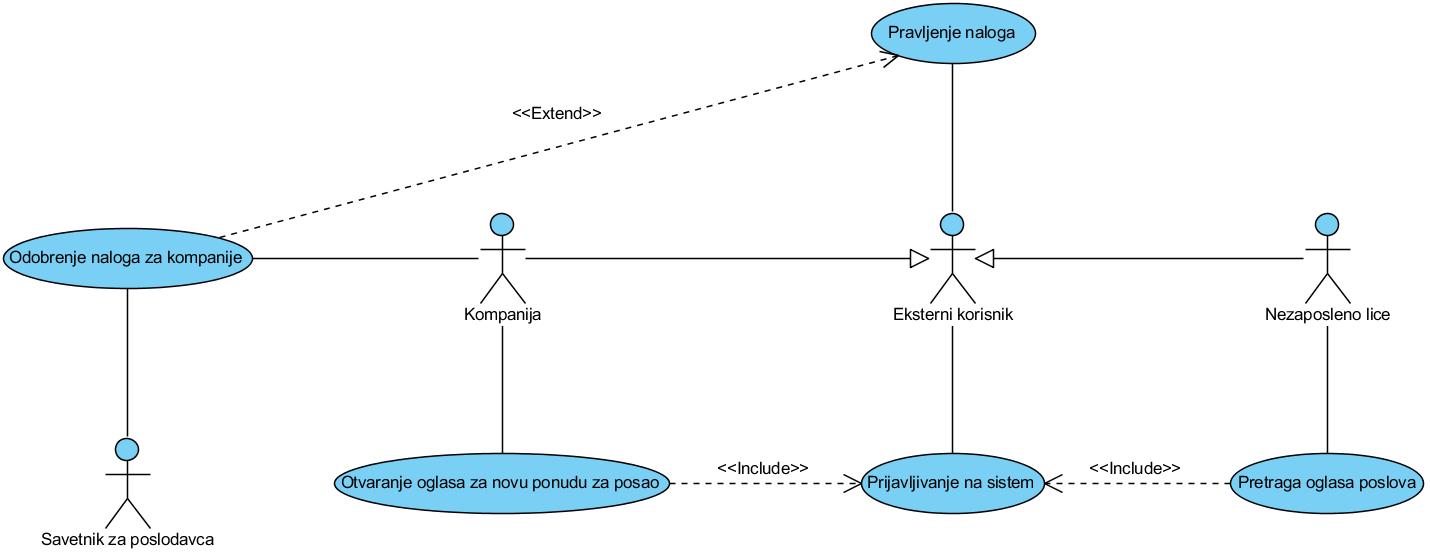
\includegraphics[width=\textwidth]{dijagrami/dijagrami-slucajeva-upotrebe/onlajn-sistem.png}
	\caption{Dijagram slu\v cajeva upotrebe procesa ''Kori\v s\' cenje onlajn sistema Nacionalne slu\v zbe''.}
	\label{dsu: koriscenje onlajn sistema nacionalne sluzbe}
\end{figure}

\subsubsection{Pravljenje naloga}
\label{su: pravljenje naloga}

\noindent U\v cesnici: Eksterni korisnik (u daljem tekstu EK)
\\
\\ Preduslovi: Ako je tip EK ''Nezaposleno lice'', onda EK ima evidentacioni karton.
\\
\\ Postuslovi: Ili je EK uspe\v sno napravio nalog ili je stanje ostalo nepromenjeno.
\\ 
\\ Glavni tok:
\begin{enumerate}
	\item EK pristupa onlajn sistemu Nacionalne slu\v zbe.
	\item Sistem prikazuje po\v cetnu stranu \ref{}.
	\item EK bira opciju ''Registracija novog korisnika''.
	\item U zavisnosti od tipa EK, Sistem prikazuje odgovaraju\' ci formular.
	\item EK popunjava formular.
	\item EK bira opciju ''Sa\v cuvaj i nastavi''.
	\item Sistem, na osnovu unetih podataka, proverava da li ve\'c postoji takav korisnik.
	\item Sistem ustanovljava da postoji takav korisnik.
	\begin{enumerate}
		\item Sistem prikazuje poruku sa obave\v stenjem i nudi EK opciju da promeni \v lozinku (ukoliko ju je zaboravio).
		\item EK bira da li \v zeli da promeni lozinku.
		\item EK bira da promeni lozinku.
		\begin{enumerate}
			\item Sistem tra\v zi od EK da unese email adresu.
			\item NK unosi email adresu i potvr\dj uje unos.
			\item Sistem obave\v stava EK da mu je poslata nova lozinka na email adresu.
			\item Slu\v caj upotrebe se zavr\v sava.
		\end{enumerate}
		\item EK bira da ne promeni lozinku, pa se prelazi na korak 2.
	\end{enumerate}
	\item Sistem ustanovljava da ne postoji takav korisnik, pa se prelazi na korak 10.
	\item Sistem utvr\dj uje tip EK.
	\item Sistem je utvrdio da je tip EK ''Nezaposleno lice'', pa se prelazi na korak 13.
	\item Sistem je utvrdio da je tip EK ''Kompanija''.
	\begin{enumerate}
		\item Prelazi se na slu\v caj upotrebe \ref{su: odobrenje naloga za kompanije}.
		\item Po zavr\v setku slu\v caja upotrebe, sistem obave\v stava EK da \' ce mu odgovor sti\' ci na email.
		\item Slu\v caj upotrebe se zavr\v sava.
	\end{enumerate}
	\item Sistem otvara novi nalog sa unetim podacima, a zatim \v salje poruku na unetu email adresu za potvr\dj ivanje.
	\item Sistem obave\v stava EK da je nalog uspe\v sno otvoren i da treba da potvrdi otvaranje naloga na email-u.
	\item Kada EK potvrdi otvaranje naloga na email-u, sistem mu prikazuje obave\v stenje da je otvaranje naloga kompletirano.
\end{enumerate}

\noindent Alternativni tokovi: 
\begin{description}
	\item[A1. Nedostupnost sistema] ~\\
	Ukoliko u bilo kom od koraka 1--4 Glavnog toka ne do\dj e do prikaza korisni\v ckog interfejsa (na primer, zbog sporog interneta), EK mo\v ze da sa\v ceka, pa da poku\v sa ponovo, ili da odustane od pravljenja naloga.
	
	\item[A2. Neispravnost unetih podataka] ~\\
	Ukoliko u koraku 6 Glavnog toka sistem utvrdi da neki podatak nije validan ili neko obavezno polje nije popunjeno, sistem generi\v se poruku o gre\v sci i zahteva od EK da ispravno popuni formu. Izvr\v savanje se nastavlja u koraku 5 Glavnog toka.
\end{description}

\subsubsection{Odobrenje naloga za kompanije}
\label{su: odobrenje naloga za kompanije}

\noindent U\v cesnici: Kompanija (u daljem tekstu K), Savetnik za poslodavce (u daljem tekstu SP)
\\
\\ Preduslovi: SP ima pristup sistemu i autorizovan je. K ima li\v cnu kartu. Ukoliko je slu\v caj upotrebe pokrenut iz slu\v caja upotrebe ''Pravljenje naloga'', onda su dostupne informacije iz formulara koji se popunjava u tom slu\v caju upotrebe (formular \ref{}).
\\
\\ Postuslovi: Ili je K uspe\v sno odobreno pravljenje naloga ili je zabele\v zen poziv za saradnju ili je stanje ostalo nepromenjeno i izdata je poruka o gre\v sci.
\\ 
\\ Glavni tok:
\begin{enumerate}
	\item Sistem proverava da li je ostvarena saradnja izme\dj u K i Nacionalne slu\v zbe.
	\item Sistem je ustanovio da je ostvarena saradnja, pa se prelazi na korak 4.
	\item Sistem je ustanovio da nije ostvarena saradnja.
	\begin{enumerate}
		\item Sistem nudi K opciju da podnese zahtev za saradnju.
		\item K bira da podnese zahtev za saradnju.
		\begin{enumerate}
			\item Sistem tra\v zi od K da unese broj li\v cne karte.
			\item K unosi broj li\v cne karte.
			\item Sistem automatski pronalazi SP koji \' ce biti zadu\v zen za K.
			\item Sistem bele\v zi novog poslodavca (na osnovu podataka iz formulara) i zadu\v zuje prona\dj enog SP za K.
			\item Prelazi se na korak 4.
		\end{enumerate}
		\item K bira da ne podnese zahtev sa saradnju, pa se slu\v caj upotrebe zavr\v sava. Ukoliko je slu\v caj upotrebe pokrenut iz slu\v caja upotrebe ''Pravljenje naloga'', onda se i taj slu\v caj upotrebe zavr\v sava.
	\end{enumerate}
	\item Sistem pronalazi SP koji je zadu\v zen za K.
	\item Sistem \v salje novi zahtev SP za autorizacijom novog naloga.
	\item SP proverava da li je zahtev u skladu sa protokolom.
	\item SP ustanovljava da zahtev jeste u skladu sa protokolom.
	\begin{enumerate}
		\item SP autorizuje zahtev.
		\item Prelazi se na korak 9.
	\end{enumerate}
	\item SP ustanovljava da zahtev nije u skladu sa protokolom.
	\begin{enumerate}
		\item SP odbija zahtev, i popunjava polje sa obrazlo\v zenjem.
		\item Sistem generi\v se poruku koja se \v salje na unetu email adresu, a koja uklju\v cuje obave\v stenje da je zahtev odbijen i obrazlo\v zenje.
		\item Slu\v caj upotrebe se zavr\v sava.
	\end{enumerate}
	\item Sistem otvara novi nalog sa unetim podacima, a zatim \v salje poruku na unetu email adresu za potvr\dj ivanje.
	\item Kada K potvrdi otvaranje naloga na email-u, sistem joj prikazuje obave\v stenje da je otvaranje naloga kompletirano.
\end{enumerate}

\noindent Alternativni tokovi: 
\\/

\subsubsection{Prijavljivanje na sistem}
\label{su: prijavljivanje na sistem}

\subsubsection{Pretraga oglasa poslova}
\label{su: pretraga oglasa poslova}

\subsubsection{Otvaranje oglasa za novu ponudu za posao}
\label{su: otvaranje oglasa za novu ponudu za posao}

\newpage
\subsection{Redovno javljanje}

Redovno javljanje predstavlja postupak dolaska nezaposlenog lica u Nacionalnu slu\v zbu radi vo\dj enja redovne evidencije o teku\' cem stanju. Nezaposleno lice je u obavezi da se na svaka 3 meseca javi u Nacionalnoj slu\v zbi, i da izvesti zaposlene koji posreduju u zapo\v sljavanju o svom trenutnom statusu.\\

U zavisnosti od nivoa izve\v stavanja nezaposleno lice mo\v ze da bira na\v cin redovnog javljanja, i to:
\begin{itemize}
	\item ukoliko nema potrebu za dodatnim uslugama Nacionalne slu\v zbe, bira jedno od naredna dva:
	\begin{itemize}
		\item Javljanje na \v salteru (slu\v caj upotrebe \ref{su: javljanje na salteru}), ili
		\item Javljanje putem interneta (slu\v caj upotrebe \ref{su: javljanje putem interneta}).
	\end{itemize}
	
	\item ukoliko ima potrebu za dodatnim uslugama Nacionalne slu\v zbe, onda bira Javljanje kod savetnika (slu\v caj upotrebe \ref{su: javljanje kod savetnika}).
\end{itemize}

Unapre\dj enje trenutnog re\v senja predstavlja Javljanje putem interneta. Ovim slu\v cajem upotrebe se uvodi novi deo onlajn sistema Nacionalne slu\v zbe, radi olak\v savanja procesa Redovno Javljanje nezaposlenih lica koji nemaju dodatne potrebe za uslugama Nacionalne slu\v zbe. Doprinosi ovog unapre\dj enja su:
\begin{itemize}
	\item smanjenje reda \v cekanja u Nacionalnoj slu\v zbi,
	\item usmeravanje rada \v salterskog slu\v zbenika na druge (zna\v cajnije) radne aktivnosti i zadatke, i
	\item obavljanje procesa Redovno javljanje iz komfornosti doma.
\end{itemize}

\subsubsection{Javljanje na \v salteru}
\label{su: javljanje na salteru}

\noindent U\v cesnici: Nezaposleno lice (u daljem tekstu NL), \v salterski slu\v zbenik (u daljem tekstu \v SS)
\\
\\ Preduslovi: NL ima evidentacioni karton. \v SS je ulogovan na sistem. 
\\
\\ Postuslovi: Ili je uspe\v sno zabele\v zeno javljanje NL-a ili je NL obave\v sten o svom stanju.
\\ 
\\ Glavni tok:
\begin{enumerate}
	\item NL prilazi automatu i bira opciju ''Redovno javljanje''.
	\item Automat bele\v zi da je opcija ''Redovno javljanje'' odabrana, ra\v cuna naredni broj u redu \v cekanja za tu opciju, i \v stampa papir sa brojem.
	\item NL uzima broj i \v ceka svoj red.
	\item Kada do\dj e na red, NL prilazi \v salteru, zahteva od \v SS da prijavi njegov dolazak, i predaje \v SS-u svoj evidentacioni karton.
	\item \v SS pronalazi NL-a u sistemu.
	\item \v SS unosi u sistem da je NL do\v sao na redovno javljanje.
	\item \v SS zakazuje slede\' ce javljanje i vra\' ca NL-u evidentacioni karton.
\end{enumerate}

\noindent Alternativni tokovi: 
\begin{description}
	\item[A1. Pad sistema] ~\\
	Ukoliko se u bilo kom koraku Glavnog toka dogodi pad sistema na kojem radi \v SS, \v SS ponovo pokre\'ce sistem i prijavljuje se na njega. Prelazi se na korak 5 Glavnog toka.
	
	\item[A2. Status NL-a je ''zamrznut''] ~\\
	Ukoliko u koraku 5 Glavnog toka sistem prika\v ze da je status NL-a ''zamrznut'', \v SS obave\v stava NL-a o njegovom statusu, i slu\v caj upotrebe se zavr\v sava.
\end{description}

\subsubsection{Javljanje putem interneta}
\label{su: javljanje putem interneta}

\subsubsection{Javljanje kod savetnika}
\label{su: javljanje kod savetnika}
\subsection{Posredovanje u zapo\v sljavanju}

Poslodavac \v zeli da zaposli radnika preko NSZ. On dolazi u slu\v zbu i na \v salteru mu ka\v zu da moraju da ga registruju u njihovu bazu poslodavaca. Poslodavac se registruje i nakon toga objavljuje oglas za nepopunjeno radno mesto u njegovoj kompaniji. Daje opis radnog mesta i uslove koje radnik mora da ispuni. Nakon toga poslodavac zapo\v sljava radnika i pravi se izve\v staj o realizaciji konkursa. 


\subsubsection{Slu\v caj upotrebe: Registracija poslodavca}

\noindent Učesnici: Poslodavac, šalterski službenik (u daljem tekstu \v SS).
\\
\\ Preduslovi: Poslodavac ima ličnu kartu.
\\
\\ Postuslovi: Poslodavac je uspešno registrovan.
\\
\\ Glavni tok:
\begin{enumerate}
\item Poslodavac prilazi automatu i bira opciju ''Registracije i verifikacije kompanije''.
	\item Automat bele\v zi da je opcija ''Registracije i verifikacije kompanije'' odabrana, ra\v cuna naredni broj u redu \v cekanja za tu opciju, i \v stampa papir sa brojem.
	\item Poslodavac uzima broj i \v ceka svoj red.
	\item Kada do\dj e na red, poslodavac prilazi \v salteru i zahteva od \v SS da ga registruje u sistemu.
	\item \v SS tra\v zi od poslodavca da mu preda li\v cnu kartu.
	\item Poslodavac predaje ličnu kartu. 
	\item \v SS daje poslodavcu formular za prijavu.
    \item Poslodavac popunjava prijavu, a zatim je vra\v ca SS-u.
	\item \v SS unosi informacije sa prijave u sistem.
	\item \v SS vra\' ca ličnu kartu poslodavcu.
	\item Prelazi se na slu\v caj upotrebe \ref{su: razgovor sa poslodavcem}.
\end{enumerate}

\noindent Alternativni tok: /

\subsubsection{Slu\v caj upotrebe: Objava konkursa}
\label{su: razgovor sa poslodavcem}

\noindent Učesnici: Poslodavac, savetnik za rad sa poslodavcima (u daljem tekstu savetnik).
\\
\\ Preduslovi: Poslodavac ima ličnu kartu i registrovan je u sistem.
\\
\\ Postuslovi: Konkurs je objavljen.
\\
\\ Glavni tok:
\begin{enumerate}
\item Poslodavac dolazi kod savetnika u kancelariju i saopštava mu da želi da zaposli radnika.
\item Savetnik traži od poslodavca da mu da ličnu kartu.
\item Poslodavac daje savetniku ličnu kartu.
\item Savetnik na osnovu podataka sa lične karte traži poslodavca u sistemu.
\item Savetnik traži od poslodavca da navede detalje o radnom mestu.
\item Poslodavac saopštava savetniku detalje o radnom mestu.
\item Savetnik unosi informacije u sistem.
\item Savetnik daje poslodavcu da popuni formular o konkursu na radno mesto.
\item Poslodavac popunjava formular, a zatim ga vraća savetniku.
\item Savetnik prosleđuje informacije svim nezaposlenima koji zadovoljavaju kriterijume iz konkursa. Slučaj upotrebe se završava.
\end{enumerate}

\subsubsection{Slu\v caj upotrebe: Realizacija konkursa}

\noindent U\v cesnici: Poslodavac, savetnik za rad sa poslodavcima (u daljem tekstu savetnik).
\\
\\ Preduslovi: Poslodavac ima dokaz o zapošljavanju nezaposlenog lica.
\\
\\ Postuslovi: Poslodavac je zaposlio nezaposleno lice i kompletiran je izve\v staj o realizaciji konkursa.
\\
\\ Glavni tok:
\begin{enumerate}
\item Poslodavac dolazi kod savetnika u kancelariju i predaje mu dokaz o zapošljavanju lica sa evidencije NSZ.
\item Savetnik pronalazi nezaposleno lice u sistemu i skida ga sa evidencije.
\item Savetnik daje poslodavcu da popuni formu o realizaciji konkursa.
\item Poslodavac popunjava  formu o realizaciji konkursa i predaje je savetniku.
\item Savetnik realizuje konkurs i uklanja ga iz sistema.
\item Savetnik vraća dokaz o zapošljavanju  poslodavcu, slučaj upotrebe se završava.
\end{enumerate}

\begin{mylandscape}
	\subsubsection{BPMN dijagrami}
	
	\begin{figure}[H]
		\centering
		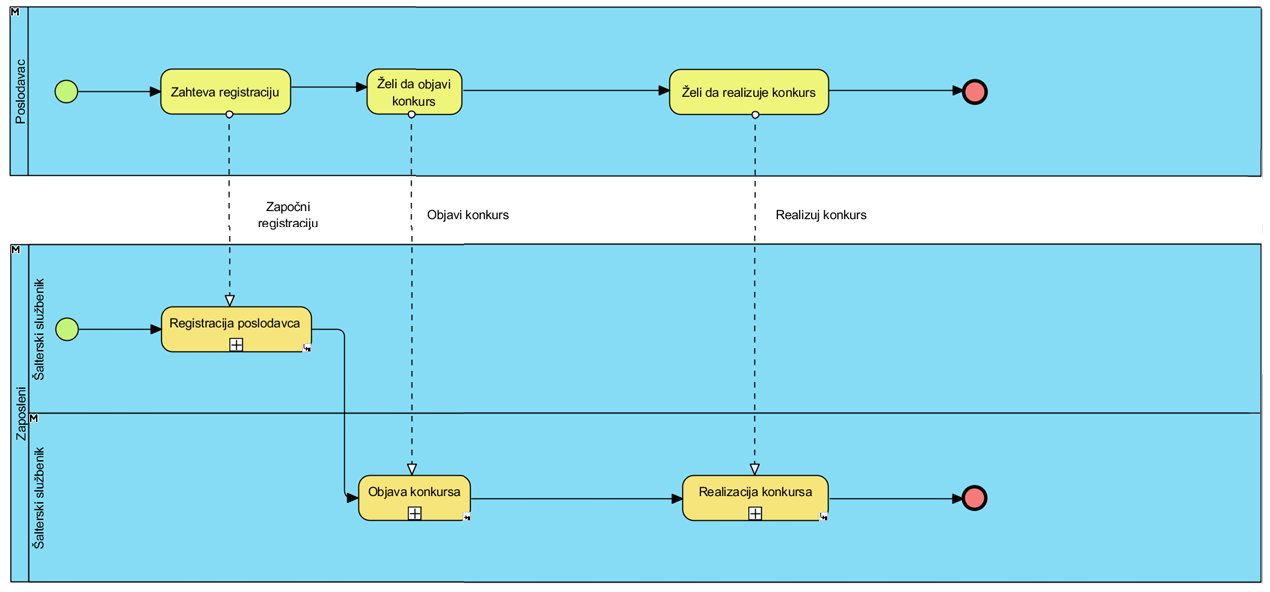
\includegraphics[width=0.7\paperwidth]{dijagrami/bpmn-dijagrami/bpmn-7.png}
		\caption{BPMN dijagram procesa ''Posredovanje u zapo\v sljavanju''.}
		\label{bpmnd: posredovanje u zaposljavanju}
	\end{figure}
	
	\newpage
	
	\begin{figure}[H]
		\centering
		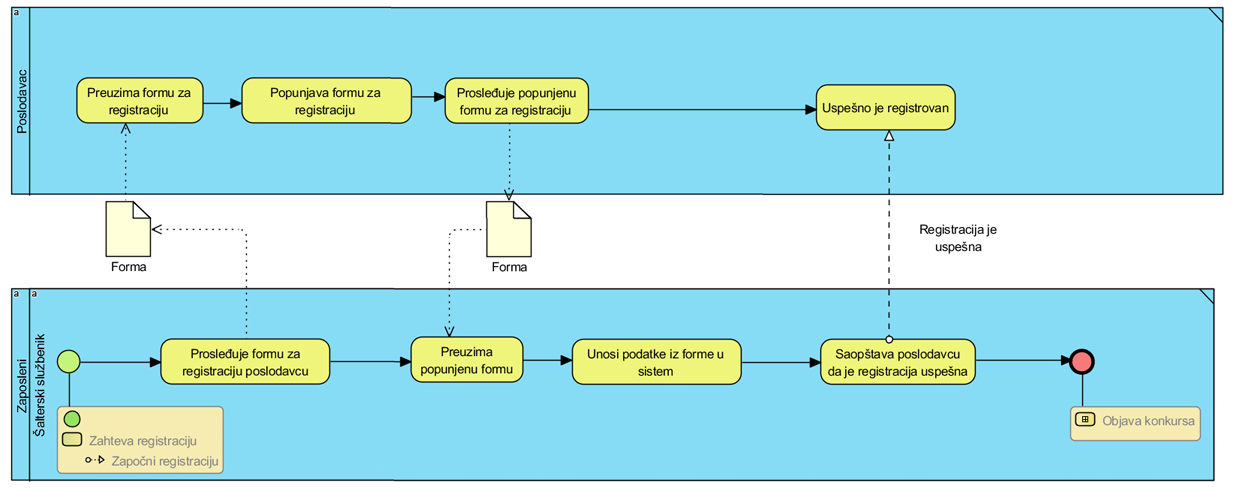
\includegraphics[width=0.7\paperwidth]{dijagrami/bpmn-dijagrami/bpmn-8.png}
		\caption{BPMN dijagram potprocesa ''Registracija poslodavca'' procesa ''Posredovanje u zapo\v sljavanju'' (\ref{bpmnd: posredovanje u zaposljavanju}).}
	\end{figure}

	\newpage
	
	\begin{figure}[H]
		\centering
		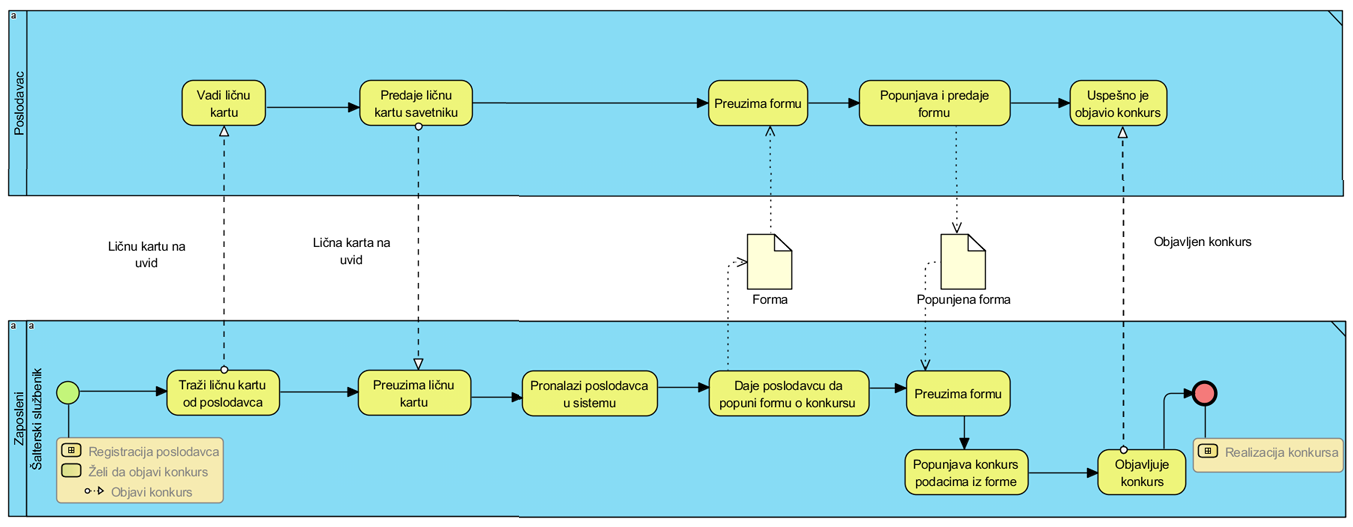
\includegraphics[width=0.7\paperwidth]{dijagrami/bpmn-dijagrami/bpmn-9.png}
		\caption{BPMN dijagram potprocesa ''Objava konkursa'' procesa ''Posredovanje u zapo\v sljavanju'' (\ref{bpmnd: posredovanje u zaposljavanju}).}
	\end{figure}

	\newpage
	
	\begin{figure}[H]
		\centering
		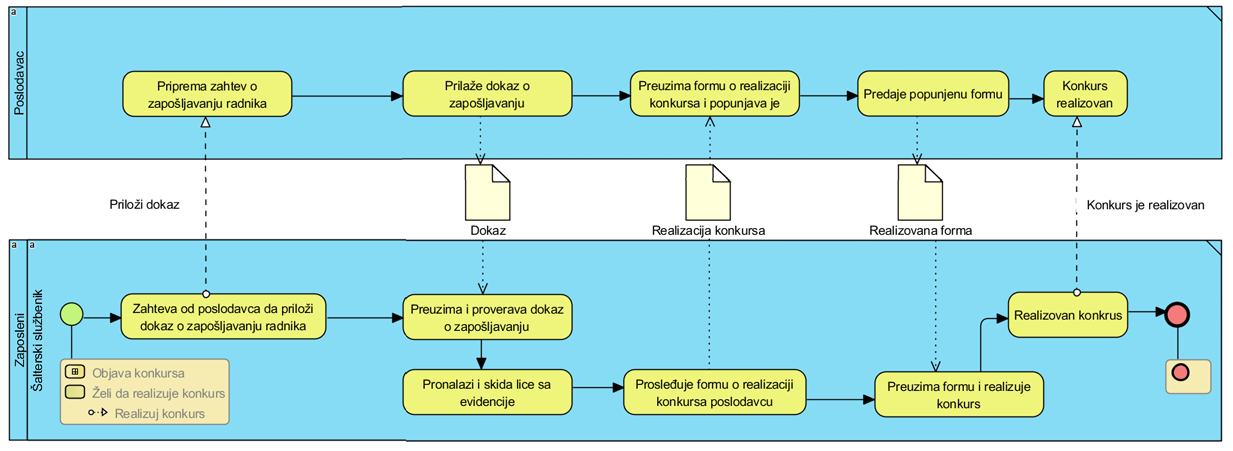
\includegraphics[width=0.7\paperwidth]{dijagrami/bpmn-dijagrami/bpmn-10.png}
		\caption{BPMN dijagram potprocesa ''Realizacija konkursa'' procesa ''Posredovanje u zapo\v sljavanju'' (\ref{bpmnd: posredovanje u zaposljavanju}).}
	\end{figure}
	
\end{mylandscape}
\subsection{Nov\v cana naknada}

Nezaposleno lice dolazi u Nacionalnu slu\v zbu za zapo\v sljavanje radi ostvarivanja prava na nov\v canu naknadu. Kako bi nezaposleno lice ostvarilo pravo na nov\v canu naknadu ono mora da se prvo prijavi za ostvarivanje iste.
\\
Nakon \v sto se prijavi za ostvarivanje prava na nov\v canu naknadu, nezaposleno lice ide kod upravnog referenta da mu preda potrebnu dokumentaciju.
\\ Predata dokumenta prosle\dj uju se zajedno sa prijavom pravnom licu koje na osnovu zakonskih odredbi i priložene dokumentacije odlu\v cuje da li je nezaposleno lice ostvarilo pravo na nov\v canu naknadu ili nije.
\\
Odluka se prosle\dj uje kod direktora na overu i zatim u pisarnicu odakle se \v salje po\v stom nezaposlenom licu.

\subsubsection{Prijava za ostvarivanja prava na nov\v canu naknadu}

\noindent Učesnici: Nezaposleno lice (u daljem tekstu NL), šalterski službenik (u daljem tekstu ŠS)
\\
\\ Preduslovi: NL ima ličnu kartu.
\\
\\ Postuslovi: Prijava je popunjena i prosleđena upravnom referentu.
\\
\\ Glavni tok:
\begin{enumerate}
\item NL prilazi automatu i bira opciju ''Prijava za novčanu naknadu''.
\item Automat bele\v zi da je opcija ''Prijava za novčanu naknadu'' odabrana, ra\v cuna naredni broj u redu \v cekanja za tu opciju, i \v stampa papir sa brojem.
\item NL uzima broj i \v ceka svoj red.
	\item Kada do\dj e na red, NL prilazi evidencionom pultu i zahteva od \v SS da ga prijavi za novčanu naknadu.
	\item \v SS otvara formular za prijavu.
	\item \v SS tra\v zi od NL da mu preda li\v cnu kartu.
	\item NL predaje li\v cnu kartu.
    \item \v SS pronalazi NL u sistemu.
	\item \v SS daje NL-u da popuni Zahtev za ostvarivanje prava na novčanu naknadu.
	\item NL popunjava Zahtev za ostvarivanje prava na novčanu naknadu, a zatim ga vra\v ca SS-u.
	\item \v SS vra\v ca ličnu kartu NL-u i upućuje ga kod upravnog referenta.
	\item Prelazi se na slu\v caj upotrebe \ref{su: prvo javljanje savetniku}.
\end{enumerate}

\begin{description}
	\item[A1. Nezaposleno lice nije prijavljeno na evidenciju] ~\\
	Ukoliko u koraku 8. Glavnog toka ŠS ne može da nađe NL u sistemu, zaključuje da NL nije prijavljeno na evidenciju tržišta rada i prelazi se na slučaj upotrebe \ref{su: prijava}.
\end{description}

\subsubsection{Kompletiranje dokumentacije}
\label{su: kompletiranje dokumentacije}

\noindent Učesnici: Nezaposleno lice (u daljem tekstu NL), upravni referent (u daljem tekstu UR).
\\
\\ Preduslovi: NL je popunio Zahtev za ostvarivanje prava na novčanu naknadu.
\\
\\ Postuslovi: UR je kompletirao dokumentaciju i prosledio je pravnom licu.
\\
\\ Glavni tok:
\begin{enumerate}
\item NL dolazi kod UR-a u kancelariju i predaje mu Zahtev za ostvarivanje prava na novčanu naknadu.
\item UR pronalazi NL u sistemu i dopunjava zahtev podacima iz evidencije.
\item UR traži od NL-a da mu preda potrebnu dokumentaciju.
\item NL-e predaje UR-u potrebnu dokumentaciju.
\item UR preuzima dokumentaciju i zahtev i šalje pravnom licu na tumačenje.
\item Prelazi se na slu\v caj upotrebe \ref{su: resenje}.
\end{enumerate}

\subsubsection{Donošenje rešenja o novčanoj naknadi}
\label{su: resenje}

\noindent Učesnici: Pravno lice.
\\
\\ Preduslovi: Upravni referent je predao Zahtev za ostvarivanje prava na novčanu naknadu i potrebnu dokumentaciju nezaposlenog lica pravnom licu.
\\
\\ Postuslovi: Nezaposleno lice je ili dobilo pravo na novčanu naknadu ili je odbijeno.
\\
\\ Glavni tok:
\begin{enumerate}
\item Pravno lice prima Zahtev za ostvarivanje prava na novčanu naknadu i potrebnu dokumentaciju.
\item Pravno lice proverava da li je sve ispravno popunjeno.
\item \begin{enumerate}
\item Pravno lice tumači zakon i na osnovu zakona i potrebne dokumentacije odobrava novčanu naknadu nezaposlenom licu.
\item Pravno lice tumači zakon i na osnovu zakona i potrebne dokumentacije ne odobrava novčanu naknadu nezaposlenom licu.
\end{enumerate}
\item Pravno lice prosleđuje rešenje o novčanoj naknadi direktoru na overu.
\item Prelazi se na slu\v caj upotrebe \ref{su: gde je pecat}.
\end{enumerate}

\begin{description}
\item [A1. Nezaposleno lice nije predalo svu potrebnu dokumentaciju] ~\\
	U koliko u koraku 2. Glavnog toka primeti da fali neophodna dokumentacija pismenim putem obaveštava nezaposleno lice da donese upravnom referentu nedostajuću dokumentaciju. Prelazi se na slučaj upotrebe \ref{su: kompletiranje dokumentacije}.
\end{description}


\subsubsection{Zaključivanje rešenja}
\label{su: gde je pecat}

\noindent Učesnici: direktor.
\\
\\ Preduslovi: Pravno lice je donelo rešenje o novčanoj naknadi i predalo ga direktoru.
\\
\\ Postuslovi: Rešenje o novčanoj naknadi je overeno.
\\
\\ Glavni tok:
\begin{enumerate}
\item Direktor preuzima rešenje o novčanoj naknadi.
\item Direktor analizira rešenje o novčanoj naknadi.
\item Direktor overava rešenje o novčanoj naknadi i prosleđuje ga pisarnici.
\item Prelazi se na slu\v caj upotrebe \ref{su: pisarnica}.
\end{enumerate}


\subsubsection{Slanje rešenja o novčanoj naknadi nezaposlenom licu}
\label{su: pisarnica}

\noindent Učesnici: Referent prijema i ekspedicije pošte (u daljem tekstu RPEP).
\\
\\ Preduslovi: Direktor je overio rešenje o novčanoj naknadi i prosledio ga pisarnici.
\\
\\ Postuslovi: Rešenje o novčanoj naknadi je poslato nezaposlenom licu.
\\
\\ Glavni tok:
\begin{enumerate}
\item RPEP preuzima overeno rešenje o novčanoj naknadi.
\item RPEP pakuje rešenje u kovertu.
\item RPEP čita adresu nezaposlenog lica iz sistema.
\item RPEP šalje overeno rešenje o novčanoj naknadi na pročitanu adresu.
\end{enumerate}


\subsection{Administracija sistema}

Administracija sistema odnosi se na dodavanje novih zaposlenih u Nacionalnoj slu\v zbi u sistem, odnosno pravljenje novih naloga, kako bi mogli da mu pristupaju. Tako\dj e, podrazumeva brisanje korisnika iz sistema koji vi\v se ne rade u slu\v zbi. Jo\v s jedan postupak koji se uklju\v cuje u ovaj slu\v caj upotrebe, a mo\v zda i najva\v zniji, je pravljenje backup-a baze podataka.

\begin{figure}[H]
	\centering
	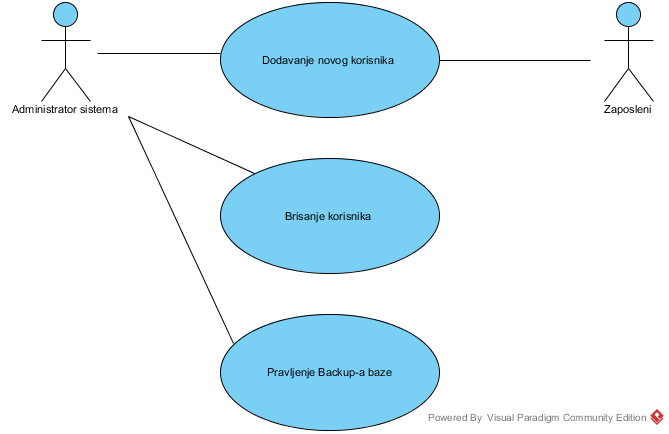
\includegraphics[width=0.8\textwidth]{dijagrami/dijagrami-slucajeva-upotrebe/administracija-sistema.png}
	\caption{Dijagram slu\v cajeva upotrebe procesa "Administracija sistema"}
	\label{dsu: administracija sistema}
\end{figure}

\subsubsection{Slu\v caj upotrebe: Dodavanje novog korisnika}

\label{su: dodavanje novog korisnika}

\noindent U\v cesnici: Administrator sistema (u daljem tekstu AS), Zaposleni (u daljem tekstu Z)
\\
\\ Preduslovi: Z je zaposlen u Nacionalnoj slu\v zbi za zapo\v sljavanje. AS ima privilegovan pristup sistemu i ulogovan je u sistem.
\\
\\ Postuslovi: AS je uspe\v sno uneo novog korisnika u sistem i Z ima mogu\' cnost logovanja na sistem i pristup podacima.
\\
\\ Glavni tok:
\begin{enumerate}
	\item Z dolazi kod AS u kancelariju i zahteva otvaranje naloga.
	\item AS bira opciju za kreiranje novog naloga.
	\item AS tra\v zi od Z da mu preda li\v cnu kartu.
	\item Z predaje li\v cnu kartu.
	\item AS proverava da li Z ve\' c ima nalog, na osnovu JMBG-a i broja li\v cne karte.
	\begin{enumerate}
		\item Ukoliko Z ve\' c ima nalog, AS odustaje od pravljenja novog naloga i slu\v caj upotrebe se ovde zavr\v sava.
		\item Ina\v ce, izvr\v savanje se nastavlja u u koraku 6.
	\end{enumerate}
	\item AS popunjava formular.
	\item AS zahteva od Z da uneste \v sifru za nalog.
	\item Z unosi \v sifru u formular.
	\item AS provera sve unete podatke i vr\v si ispravke u slu\v caju unosa pogre\v snog podatka.
	\item AS potvr\dj uje unos.
	\item AS \v stampa potvrdu o uspe\v sno napravljenom nalogu.
	\item AS vra\' ca li\v cnu kartu i predaje potvrdu o nalogu. 
	
\end{enumerate}

\noindent Alternativni tok:
\begin{description}
	\item[A1. Pad sistema] ~\\
	Ukoliko se u bilo kom koraku Glavnog toka dogodi pad sistema na kojem radi AS, AS ponovo pokre\'ce sistem i prijavljuje se na njega.
	\begin{enumerate}
		\item AS proverava da li je formular sa\v cuvan.
		\item Ukoliko jeste, prelazi se na korak 8 Glavnog toka.
		\item Ina\v ce, prelazi se na korak 6 Glavnog toka.
	\end{enumerate}
	\item[A2. Neuspe\v san unos] ~\\
	Ukoliko u koraku 9 Glavnog toka sistem prijavi gre\v sku pri \v cuvanju informacija, AS poku\v sava ponovo. Izvr\v savanje se nastavlja u koraku 5 Glavnog toka.
\end{description}


\subsubsection{Slu\v caj upotrebe: Brisanje korisnika}

\label{su: brisanje korisnika}

\noindent U\v cesnici: Administrator sistema (u daljem tekstu AS)
\\
\\ Preduslovi: AS ima privilegovan pristup sistemu i ulogova je u sistem. AS je primio zahtev za brisanje korisnika.
\\
\\ Postuslovi: Korisnik je uspe\v sno obrisan iz sistema ili je stanje sistema nepromenjeno.
\\
\\ Glavni tok:
\begin{enumerate}
	\item AS otvara zahtev za brisanje korisnika.
	\item AS pronalazi korinsika u sistemu.
	\item AS bira opciju "Obri\v si korisnika".
	\item Sistem zahteva od AS da potvrdi akciju koju \v zeli da izvr\v si.
	\begin{itemize}
		\item Ukoliko AS pritisne ''Da'', sistem vr\v si operaciju brisanja.
		\item Ukoliko AS pritisne ''Ne'' nikakve promene nisu na\v cinjene.
	\end{itemize}
\end{enumerate}

\noindent Alternativni tok: /

\subsubsection{Slu\v caj upotrebe: Back-up baze podataka}


\label{su: backup}
\noindent U\v cesnici: Administrator sistema (u daljem tekstu AS)
\\
\\ Preduslovi: Sistem ispravno funkcioni\v se. AS je ulogovan na sistem i ima privilegovan pristup.
\\
\\ Postuslovi: Backup je uspe\v sno napravljen.
\\
\\ Glavni tok:
\begin{enumerate}
	\item AS proverava da li se trenutno vr\v si neka bitna obrada nad bazom.
	\begin{itemize}
		\item Ukoliko je to slu\v caj, AS \v ceka da se zavr\v si.
		\item U suprotnom, izvr\v savanje se nastavlja u koraku 2.
	\end{itemize}
	\item AS bira da li pravi standardni backup baze ili \v zeli da postavi detaljnije parametre.
	\begin{itemize}
		\item Ukoliko je odabran backup sa parametrima, AS ih pode\v sava.
		\item U suprotnom se prelazi na slede\' ci korak.
	\end{itemize}
	\item AS pokre\' ce pravljenej backup-a.
	\item AS snima backup na memorijski medijum i bele\v zi vreme kada je napravljen.
\end{enumerate}

\noindent Alternatinvni tok: /

\subsubsection{Dijagrami sekvence}

\begin{figure}[H]
	\centering
	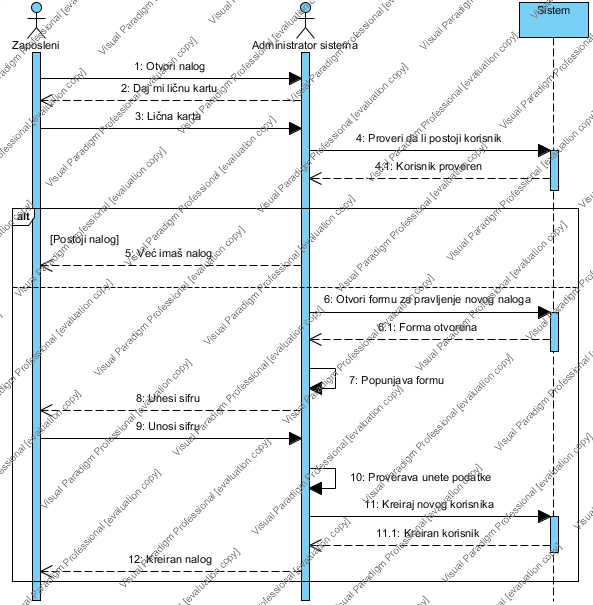
\includegraphics[width=0.6\paperwidth]{dijagrami/dijagrami-sekvence/dodavanje-novog-korisnika.png}
	\caption{Dijagram sekvence slu\v caja upotrebe ''Dodavanje novog korisnika'' (\ref{su: dodavanje novog korisnika}).}
\end{figure}

\newpage

\begin{figure}[H]
	\centering
	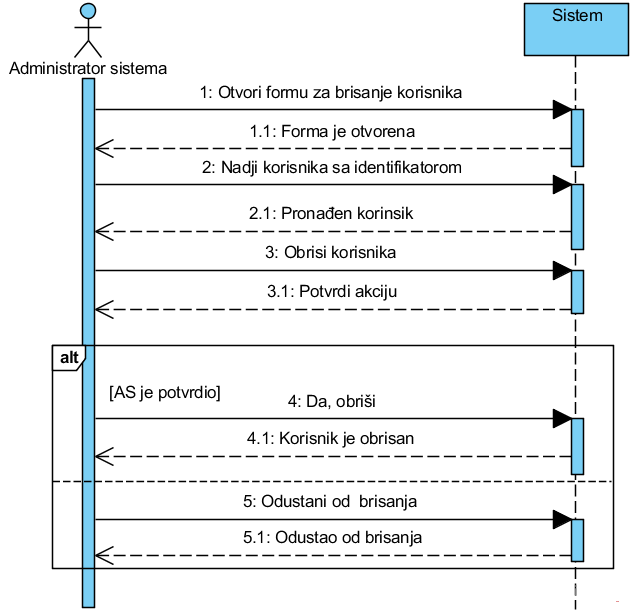
\includegraphics[width=0.7\paperwidth]{dijagrami/dijagrami-sekvence/brisanje-korisnika.png}
	\caption{Dijagram sekvence slu\v caja upotrebe ''Brisanje korisnika' (\ref{su: brisanje korisnika}).}
\end{figure}

\newpage

\begin{figure}[H]
	\centering
	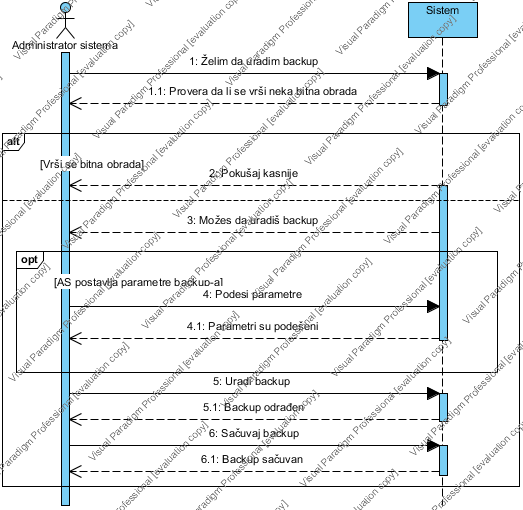
\includegraphics[width=0.95\textwidth]{dijagrami/dijagrami-sekvence/backup.png}
	\caption{Dijagram sekvence slu\v caja upotrebe ''Back-up baze podataka'' (\ref{su: backup}).}
\end{figure}
\section{Klase podataka}

Analizom slu\v cajeva upotrebe, uo\v cene su slede\' ce grupe podataka:

\begin{itemize}
	\item Zaposleni u Nazionalnoj slu\v zbi za zapo\v sljavanje
	\item Nezaposlena lica na evidenciji
		\begin{itemize}
			\item  li\v cni podaci o nezaposlenom licu
			\item podaci o ve\v stinama nezaposlenog lica
			\item podaci o prethodnim zaposlenjima nezaposlenog lica
			\item podaci o javljanju
			\item podaci o radnoj sposobnosti
			\item podaci o nov\v canoj naknadi 
			\item podaci o nalogu za online javljanje
		\end{itemize}
	\item Poslodavci
		\begin{itemize}
			\item podaci o kompaniji
			\item podaci o oglasima i konkursima za poslove
			\item podaci o potrebnim profilima ljudi
			\item podaci o nalogu za online otvaranje oglasa
		\end{itemize}
	\item Zanimanja
		\begin{itemize}
			\item podaci o zanimanjima
			\item podaci o stru\v cnoj spremi
		\end{itemize}
\end{itemize}

\begin{mylandscape}
\subsection{Dijagram klasa podataka}

\begin{figure}[H]
	\centering
	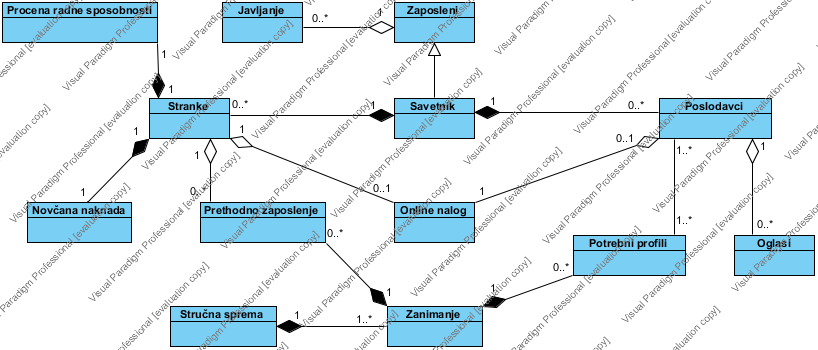
\includegraphics[width=0.8\paperwidth]{dijagrami/dijagrami-klasa/dijagrami-klasa.png}
	\caption{Dijagram klasa}
	\label{dk}
\end{figure}
\end{mylandscape}


\subsection{Podaci o zaposlenima u Nacionalnoj slu\v zbi za zapo\v sljavanje}

Klasa "Zaposleni" sadr\v zi sve potrebne podatke o zaposlenima uklju\v cuju\' ci:
\begin{itemize}
	\item Ime i prezime
	\item JMBG
	\item Datum ro\dj enja
	\item Adresa stanovanja
	\item Telefon
	\item E-mail adresa
	\item Datum zaposlenja
	\item Pozicija (\v salterski slu\v zbenik, savetnik za zapo\v sljavanje, savetnik za poslodavce, administrator sistema)
	\item Plata
	\item \v Sifra (za logovanje na sistem)
\end{itemize}

\noindent Klasa ''Zaposleni'' ima slede\' ce specijalizacije: \v Salterski slu\v zbenik, Savetnik, Upravni referent, Pravno lice, Direktor

\subsection{Podaci o nezaposlenim licima na evidenciji}

Klasa "Nezaposlena lica" sadr\v i li\v cne podatke o licu, kao i podatke o zanimanju stru\v cnoj spremi.
\\
\\ Podaci o nezaposlenim licima:
\begin{itemize}
	\item Ime i prezime
	\item Broj li\v cne karte
	\item JMBG
	\item Datum ro\dj enja
	\item Pol
	\item Mesto stanovanja
	\item Op\v stina stanovanja
	\item Adresa stanovanja
	\item Ku\' cni broj
	\item Broj stana 
	\item Datum prijave na evidenciju
	\item Telefon
	\item E-mail adresa
	\item Status (aktivan, zamrznut, zaposlen)
	\item Zaduzeni savetnik (referenca na Zaposleni)
	\item Procena radne sposobnosti
\end{itemize}

\noindent Podaci o prethodnim zaposlenjima:
\begin{itemize}
	\item Naziv
	\item Opis radnog mesta
\end{itemize}

\noindent Podaci o javljanju:
\begin{itemize}
	\item Datum javljanja
	\item Online (bool vrednost koja ozna\v cava da li je javljanje obavljeno putem interneta ili li\v cno u slu\v bi)
	\item Odlazak kod savetnika (bool vrednost koja ozna\v cava da li lice \v zeli da ode i kod savetnika)
	\item Termin za odlazak kod savetnika
	\item Datum zakazanog slede\' ceg javljanja
\end{itemize}

\noindent Podaci o nov\v canoj naknadi:
\begin{itemize}
	\item Prose\v cna zarada
	\item Broj ra\v cuna
	\item \v Sifra banke - po\v ste
\end{itemize}

\noindent Podaci o nalogu za online javljanje:
\begin{itemize}
	\item E-mail
	\item Lozinka
\end{itemize}

\noindent Podaci o proceni radne sposobnosti:
\begin{itemize}
	\item Ime i prezime lekara veštaka Republi\v ckog fonda penzijskog i invalidskog osiguranja
	\item Ime i prezime specijaliste medicine rada
	\item Ime i prezime psihologa
	\item Stru\v cni radnik Nacionalne slu\v zbe za zapo\v sljavanje (referenca na Zaposleni)
	\item Prostorija
	\item Datum i vreme
\end{itemize}


\subsection{Poslodavci}
Klasa Poslodavci obuhvata sve podatke o kompanijama koje \v zele da sara\dj uju sa Nacionalnom slu\v zbom za zaposljavanje kao i o njihovim potrebama i oglasima.
\\
\\ Podaci o kompaniji:
\begin{itemize}
	\item Naziv
	\item Opis
	\item Ime i prezime vlasnika
	\item Broj li\v cne katre vlasnika
	\item Adresa
	\item Telefon
	\item E-mail adresa
	\item Veb stranica
\end{itemize}

\noindent Podaci o oglasima i konkursima za poslove:
\begin{itemize}
	\item Opis radnog mesta
	\item Pla\' ceno
	\item Suma
	\item Odobreno (bool vrednost koja ozna\v cava da li je oglas odobren ili ne)
\end{itemize}

\noindent Podaci o potrebnim profilima ljudi:
\begin{itemize}
	\item Zvanje
	\item Stru\v cna sprema
	\item Broj otvorenih pozicija
\end{itemize}

\noindent Podaci o nalogu za online otvaranje oglasa:
\begin{itemize}
	\item E-mail adresa
	\item Lozinka
\end{itemize}


\subsection{Zanimanja}
Klasa "Zanimanja" odnosi se na podatke o stru\v cnoj spremi i zvanjima koja postoje.
\\
\\ Podaci o zvanjima:
\begin{itemize}
	\item Naziv
	\item Opis
	\item Stru\v cna sprema
\end{itemize}

\noindent Podaci o stru\v cnoj spremi:
\begin{itemize}
	\item Stepen
	\item Opis
	\item Godine za stepen
	\item Godine ukupno
\end{itemize}


\thispagestyle{empty}
\begin{thebibliography}{9}
	
	\bibitem{smalkov-slajdovi}
	Malkov Sa\v sa.
	\href{http://poincare.matf.bg.ac.rs/~smalkov/nastava.master.html\#r271\_is}{\textit{Slajdovi sa predavanja na kursu Informacioni sistemi}}.
	
	\bibitem{SADM}
	Whitten Jeffrey, Bentley Lonnie.
	\textit{Systems Analysis and Design Methods, 7th Edition}.
	Irwin/McGraw--Hill Education.
	2007.
	
	\bibitem{BPMN}
	von Rosing Mark, Scheer August-Wilhelm, von Scheel Henrik.
	\href{http://www.omg.org/news/whitepapers/Business_Process_Model_and_Notation.pdf}{\textit{The Complete Business Process Handbook}}.
	2015.
	
	\bibitem{SAAD}
	Dennis Alan, Wixom Barbara, Roth Roberta
	\textit{System Analysis \& Design, 5th Edition}.
	John Wiley \& Sons, Inc.
	2012.
	
\end{thebibliography}
\addcontentsline{toc}{section}{Literatura}

\end{document}